\documentclass[]{article}
\usepackage{lmodern}
\usepackage{amssymb,amsmath}
\usepackage{ifxetex,ifluatex}
\usepackage{fixltx2e} % provides \textsubscript
\ifnum 0\ifxetex 1\fi\ifluatex 1\fi=0 % if pdftex
  \usepackage[T1]{fontenc}
  \usepackage[utf8]{inputenc}
\else % if luatex or xelatex
  \ifxetex
    \usepackage{mathspec}
  \else
    \usepackage{fontspec}
  \fi
  \defaultfontfeatures{Ligatures=TeX,Scale=MatchLowercase}
\fi
% use upquote if available, for straight quotes in verbatim environments
\IfFileExists{upquote.sty}{\usepackage{upquote}}{}
% use microtype if available
\IfFileExists{microtype.sty}{%
\usepackage{microtype}
\UseMicrotypeSet[protrusion]{basicmath} % disable protrusion for tt fonts
}{}
\usepackage[margin=1in]{geometry}
\usepackage{hyperref}
\hypersetup{unicode=true,
            pdfborder={0 0 0},
            breaklinks=true}
\urlstyle{same}  % don't use monospace font for urls
\usepackage{color}
\usepackage{fancyvrb}
\newcommand{\VerbBar}{|}
\newcommand{\VERB}{\Verb[commandchars=\\\{\}]}
\DefineVerbatimEnvironment{Highlighting}{Verbatim}{commandchars=\\\{\}}
% Add ',fontsize=\small' for more characters per line
\usepackage{framed}
\definecolor{shadecolor}{RGB}{248,248,248}
\newenvironment{Shaded}{\begin{snugshade}}{\end{snugshade}}
\newcommand{\KeywordTok}[1]{\textcolor[rgb]{0.13,0.29,0.53}{\textbf{#1}}}
\newcommand{\DataTypeTok}[1]{\textcolor[rgb]{0.13,0.29,0.53}{#1}}
\newcommand{\DecValTok}[1]{\textcolor[rgb]{0.00,0.00,0.81}{#1}}
\newcommand{\BaseNTok}[1]{\textcolor[rgb]{0.00,0.00,0.81}{#1}}
\newcommand{\FloatTok}[1]{\textcolor[rgb]{0.00,0.00,0.81}{#1}}
\newcommand{\ConstantTok}[1]{\textcolor[rgb]{0.00,0.00,0.00}{#1}}
\newcommand{\CharTok}[1]{\textcolor[rgb]{0.31,0.60,0.02}{#1}}
\newcommand{\SpecialCharTok}[1]{\textcolor[rgb]{0.00,0.00,0.00}{#1}}
\newcommand{\StringTok}[1]{\textcolor[rgb]{0.31,0.60,0.02}{#1}}
\newcommand{\VerbatimStringTok}[1]{\textcolor[rgb]{0.31,0.60,0.02}{#1}}
\newcommand{\SpecialStringTok}[1]{\textcolor[rgb]{0.31,0.60,0.02}{#1}}
\newcommand{\ImportTok}[1]{#1}
\newcommand{\CommentTok}[1]{\textcolor[rgb]{0.56,0.35,0.01}{\textit{#1}}}
\newcommand{\DocumentationTok}[1]{\textcolor[rgb]{0.56,0.35,0.01}{\textbf{\textit{#1}}}}
\newcommand{\AnnotationTok}[1]{\textcolor[rgb]{0.56,0.35,0.01}{\textbf{\textit{#1}}}}
\newcommand{\CommentVarTok}[1]{\textcolor[rgb]{0.56,0.35,0.01}{\textbf{\textit{#1}}}}
\newcommand{\OtherTok}[1]{\textcolor[rgb]{0.56,0.35,0.01}{#1}}
\newcommand{\FunctionTok}[1]{\textcolor[rgb]{0.00,0.00,0.00}{#1}}
\newcommand{\VariableTok}[1]{\textcolor[rgb]{0.00,0.00,0.00}{#1}}
\newcommand{\ControlFlowTok}[1]{\textcolor[rgb]{0.13,0.29,0.53}{\textbf{#1}}}
\newcommand{\OperatorTok}[1]{\textcolor[rgb]{0.81,0.36,0.00}{\textbf{#1}}}
\newcommand{\BuiltInTok}[1]{#1}
\newcommand{\ExtensionTok}[1]{#1}
\newcommand{\PreprocessorTok}[1]{\textcolor[rgb]{0.56,0.35,0.01}{\textit{#1}}}
\newcommand{\AttributeTok}[1]{\textcolor[rgb]{0.77,0.63,0.00}{#1}}
\newcommand{\RegionMarkerTok}[1]{#1}
\newcommand{\InformationTok}[1]{\textcolor[rgb]{0.56,0.35,0.01}{\textbf{\textit{#1}}}}
\newcommand{\WarningTok}[1]{\textcolor[rgb]{0.56,0.35,0.01}{\textbf{\textit{#1}}}}
\newcommand{\AlertTok}[1]{\textcolor[rgb]{0.94,0.16,0.16}{#1}}
\newcommand{\ErrorTok}[1]{\textcolor[rgb]{0.64,0.00,0.00}{\textbf{#1}}}
\newcommand{\NormalTok}[1]{#1}
\usepackage{graphicx,grffile}
\makeatletter
\def\maxwidth{\ifdim\Gin@nat@width>\linewidth\linewidth\else\Gin@nat@width\fi}
\def\maxheight{\ifdim\Gin@nat@height>\textheight\textheight\else\Gin@nat@height\fi}
\makeatother
% Scale images if necessary, so that they will not overflow the page
% margins by default, and it is still possible to overwrite the defaults
% using explicit options in \includegraphics[width, height, ...]{}
\setkeys{Gin}{width=\maxwidth,height=\maxheight,keepaspectratio}
\IfFileExists{parskip.sty}{%
\usepackage{parskip}
}{% else
\setlength{\parindent}{0pt}
\setlength{\parskip}{6pt plus 2pt minus 1pt}
}
\setlength{\emergencystretch}{3em}  % prevent overfull lines
\providecommand{\tightlist}{%
  \setlength{\itemsep}{0pt}\setlength{\parskip}{0pt}}
\setcounter{secnumdepth}{0}
% Redefines (sub)paragraphs to behave more like sections
\ifx\paragraph\undefined\else
\let\oldparagraph\paragraph
\renewcommand{\paragraph}[1]{\oldparagraph{#1}\mbox{}}
\fi
\ifx\subparagraph\undefined\else
\let\oldsubparagraph\subparagraph
\renewcommand{\subparagraph}[1]{\oldsubparagraph{#1}\mbox{}}
\fi

%%% Use protect on footnotes to avoid problems with footnotes in titles
\let\rmarkdownfootnote\footnote%
\def\footnote{\protect\rmarkdownfootnote}

%%% Change title format to be more compact
\usepackage{titling}

% Create subtitle command for use in maketitle
\newcommand{\subtitle}[1]{
  \posttitle{
    \begin{center}\large#1\end{center}
    }
}

\setlength{\droptitle}{-2em}

  \title{2018R1 Regression in Practice (STAT5102) Assignment 2}
    \pretitle{\vspace{\droptitle}\centering\huge}
  \posttitle{\par}
    \author{Yiu Chung WONG 1155017920}
    \preauthor{\centering\large\emph}
  \postauthor{\par}
    \date{}
    \predate{}\postdate{}
  

\begin{document}
\maketitle

\begin{Shaded}
\begin{Highlighting}[]
\NormalTok{BGSall <-}\StringTok{ }\KeywordTok{read.csv}\NormalTok{(}\StringTok{"BGSall.txt"}\NormalTok{, }\DataTypeTok{header =} \OtherTok{TRUE}\NormalTok{, }\DataTypeTok{sep =} \StringTok{" "}\NormalTok{)}
\NormalTok{BGSboys <-}\StringTok{ }\KeywordTok{read.csv}\NormalTok{(}\StringTok{"BGSboys.txt"}\NormalTok{, }\DataTypeTok{header =} \OtherTok{TRUE}\NormalTok{, }\DataTypeTok{sep =} \StringTok{" "}\NormalTok{)}
\NormalTok{BGSgirls <-}\StringTok{ }\KeywordTok{read.csv}\NormalTok{(}\StringTok{"BGSgirls.txt"}\NormalTok{, }\DataTypeTok{header =} \OtherTok{TRUE}\NormalTok{, }\DataTypeTok{sep =} \StringTok{" "}\NormalTok{)}
\NormalTok{maple <-}\StringTok{ }\KeywordTok{read.table}\NormalTok{(}\StringTok{"maple.txt"}\NormalTok{, }\DataTypeTok{header =} \OtherTok{TRUE}\NormalTok{, }\DataTypeTok{sep =} \StringTok{""}\NormalTok{, }\DataTypeTok{stringsAsFactors =} \OtherTok{TRUE}\NormalTok{)}
\end{Highlighting}
\end{Shaded}

\subsubsection{1.}\label{section}

\paragraph{{[}Berkeley Guidance Study{]} The Berkeley Guidance Study
enrolled children born in Berkeley, California, between January 1928 and
June 1929, and then measured them periodically until age eighteen
(Tuddenham and Snyder, 1954). The data we use is described in Table 1,
and the data is given in the data files BGSgirls.txt for girls only, and
BGSall.txt for boys and girls
combined.}\label{berkeley-guidance-study-the-berkeley-guidance-study-enrolled-children-born-in-berkeley-california-between-january-1928-and-june-1929-and-then-measured-them-periodically-until-age-eighteen-tuddenham-and-snyder-1954.-the-data-we-use-is-described-in-table-1-and-the-data-is-given-in-the-data-files-bgsgirls.txt-for-girls-only-and-bgsall.txt-for-boys-and-girls-combined.}

\paragraph{a. For the girls only, draw the scatterplot matrix of all the
age two variables, all the age nine variables and Soma. Write a summary
of the information in this scatterplot matrix. Also obtain the matrix of
sample correlations between the height
variables}\label{a.-for-the-girls-only-draw-the-scatterplot-matrix-of-all-the-age-two-variables-all-the-age-nine-variables-and-soma.-write-a-summary-of-the-information-in-this-scatterplot-matrix.-also-obtain-the-matrix-of-sample-correlations-between-the-height-variables}

\begin{Shaded}
\begin{Highlighting}[]
\NormalTok{my.lm <-}\StringTok{ }\ControlFlowTok{function}\NormalTok{(data, mapping, ...)\{}
\NormalTok{  p <-}\StringTok{ }\KeywordTok{ggplot}\NormalTok{(}\DataTypeTok{data =}\NormalTok{ data, }\DataTypeTok{mapping =}\NormalTok{ mapping) }\OperatorTok{+}\StringTok{ }
\StringTok{    }\KeywordTok{geom_point}\NormalTok{(}\DataTypeTok{size =} \DecValTok{2}\NormalTok{) }\OperatorTok{+}\StringTok{ }
\StringTok{    }\KeywordTok{geom_smooth}\NormalTok{(}\DataTypeTok{method =}\NormalTok{ loess, }\DataTypeTok{fill =} \StringTok{"red"}\NormalTok{, }\DataTypeTok{color =} \StringTok{"red"}\NormalTok{, }\DataTypeTok{size =} \DecValTok{1}\NormalTok{, ...) }\OperatorTok{+}
\StringTok{    }\KeywordTok{geom_smooth}\NormalTok{(}\DataTypeTok{method =}\NormalTok{ lm, }\DataTypeTok{fill =} \StringTok{"blue"}\NormalTok{, }\DataTypeTok{color =} \StringTok{"blue"}\NormalTok{, }\DataTypeTok{size =} \DecValTok{1}\NormalTok{, ...)}
\NormalTok{  p}
\NormalTok{\}}


\NormalTok{g <-}\StringTok{ }\KeywordTok{ggpairs}\NormalTok{(}
\NormalTok{        BGSgirls, }
        \DataTypeTok{columns =} \KeywordTok{c}\NormalTok{(}\DecValTok{2}\OperatorTok{:}\DecValTok{7}\NormalTok{, }\DecValTok{12}\NormalTok{),}
        \DataTypeTok{upper =} \KeywordTok{list}\NormalTok{(}\DataTypeTok{continuous =} \KeywordTok{wrap}\NormalTok{(}\StringTok{"cor"}\NormalTok{, }\DataTypeTok{size =} \DecValTok{10}\NormalTok{, }\DataTypeTok{method =} \StringTok{"spearman"}\NormalTok{)),}
        \DataTypeTok{diag =} \KeywordTok{list}\NormalTok{(}\DataTypeTok{continuous =} \KeywordTok{wrap}\NormalTok{(}\StringTok{"barDiag"}\NormalTok{, }\DataTypeTok{bins =} \KeywordTok{sqrt}\NormalTok{(}\KeywordTok{nrow}\NormalTok{(BGSgirls)))),}
        \DataTypeTok{lower =} \KeywordTok{list}\NormalTok{(}\DataTypeTok{continuous =}\NormalTok{ my.lm)}
\NormalTok{        )}

\NormalTok{g <-}\StringTok{ }\NormalTok{g }\OperatorTok{+}\StringTok{ }\KeywordTok{ggtitle}\NormalTok{(}\StringTok{"BGSgirls Age Two Correlation Matrix"}\NormalTok{) }\OperatorTok{+}\StringTok{ }
\StringTok{        }\KeywordTok{theme}\NormalTok{(}\DataTypeTok{plot.title =} \KeywordTok{element_text}\NormalTok{(}\DataTypeTok{lineheight =}\NormalTok{ .}\DecValTok{8}\NormalTok{,}
                                        \DataTypeTok{face =} \StringTok{"bold"}\NormalTok{,}
                                        \DataTypeTok{size =} \DecValTok{20}\NormalTok{), }
              \DataTypeTok{axis.title.x =} \KeywordTok{element_text}\NormalTok{(}\DataTypeTok{size =} \DecValTok{10}\NormalTok{))}

\NormalTok{g}
\end{Highlighting}
\end{Shaded}

\begin{center}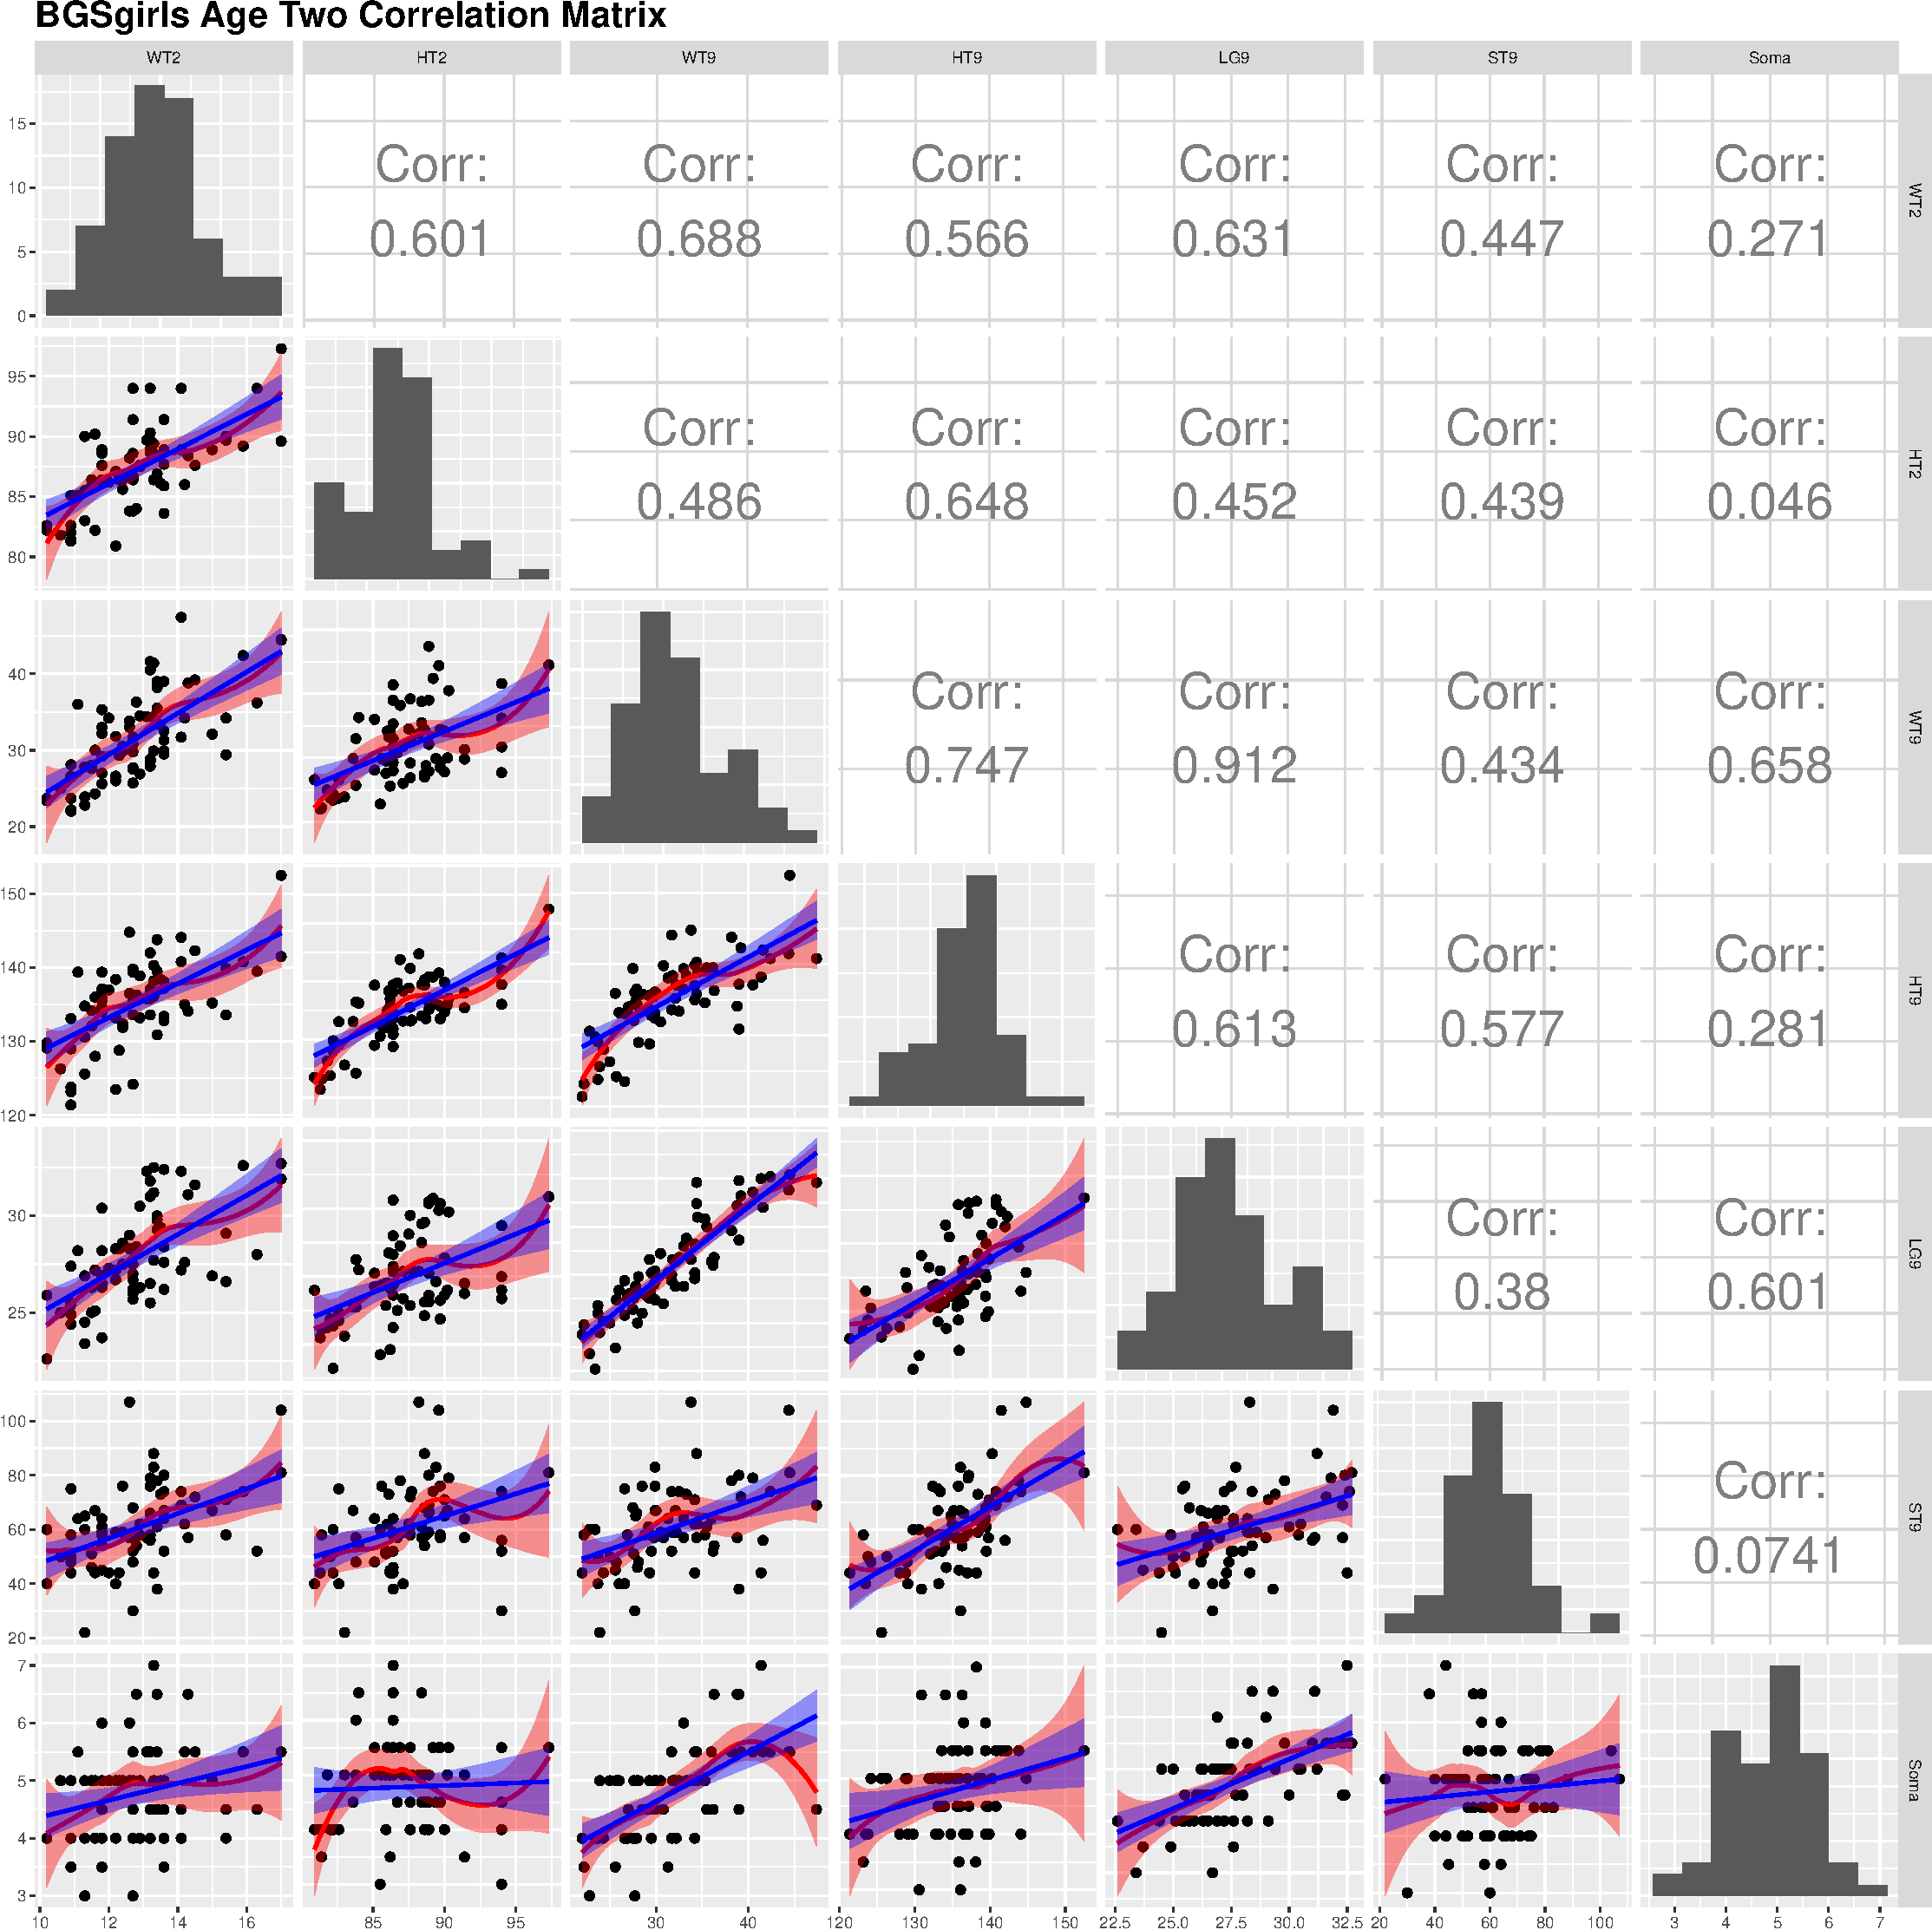
\includegraphics{Assignment_2_files/figure-latex/fig2-1} \end{center}

\begin{itemize}
\item
  \texttt{Soma} is the dependent variable to be used for the regression
  analysis. It appears to have moderate linear relations with several
  other variables such as \texttt{ST9} and \texttt{WT9}.
\item
  Each predictors look fairly normal. Although OLS regression does not
  assume normality in the predictors, non-normal data \textbf{MAY} cause
  the relationship between them and the target variable to be
  non-linear. Looking at the bottom row and comparing loess curves (red)
  to the linear regression lines (blue) of all the graphs, the
  relationships between these predictors and \texttt{Soma} are
  relatively linear, so no linear transformations is required prior to
  modelling. 
\item
  In the same row, points are scattered around fairly evenly. This means
  variance are consistent across value of \texttt{Soma} and the
  predictors. Hence heteroskedasticity not likely to exist in the
  residual terms.
\item
  Many predictors are highly correlated to each other. For example,
  \texttt{HT9} and \texttt{WT9} have correlation 0.728; \texttt{LG9} and
  \texttt{WT9} have correlation 0.904. Collinearity can also hide
  amongst the whole set of predictors instead of just two. Therefore, we
  are not safe from multicollinearity simply because other predictors
  are of lower correlation. Other metrics such as Variance Inflation
  Factor is better at simultaneously evaluating one predictor against
  all others. One must be caution of multicollinearity in this dataset
  because they reduces the precision of the estimate coefficients (by
  weakening statistical power), as well as making coefficients sensitive
  (varies greatly) under the presence of other predictors in the model.
\end{itemize}

\begin{Shaded}
\begin{Highlighting}[]
\KeywordTok{cor}\NormalTok{(BGSgirls[,}\KeywordTok{c}\NormalTok{(}\DecValTok{3}\NormalTok{, }\DecValTok{5}\NormalTok{, }\DecValTok{9}\NormalTok{)])}
\end{Highlighting}
\end{Shaded}

\begin{verbatim}
##            HT2       HT9      HT18
## HT2  1.0000000 0.7383562 0.6633351
## HT9  0.7383562 1.0000000 0.8078083
## HT18 0.6633351 0.8078083 1.0000000
\end{verbatim}

\paragraph{b. Fit the multiple linear regression model with mean
function}\label{b.-fit-the-multiple-linear-regression-model-with-mean-function}

\[
\begin{align*}
 \operatorname{E} (Soma \mid X ) = \beta_0 + \beta_1 HT2 + \beta_2 WT2 + \beta_3 HT9 + \beta_4 WT9 + \beta_5 ST9   \\
\end{align*}
\]

\paragraph{\texorpdfstring{based on BGSall.txt. Find
\emph{\(\sigma^2\)}, \emph{\(R^2\)}, the overall analysis of variance
table and overall F-test. Compute the t-statistics to be used to test
each of the \emph{\(\beta_{j}\)} to be zero against two-sided
alternatives. Explicitly state the hypotheses tested and the
conclusions.}{based on BGSall.txt. Find \textbackslash{}sigma\^{}2, R\^{}2, the overall analysis of variance table and overall F-test. Compute the t-statistics to be used to test each of the \textbackslash{}beta\_\{j\} to be zero against two-sided alternatives. Explicitly state the hypotheses tested and the conclusions.}}\label{based-on-bgsall.txt.-find-sigma2-r2-the-overall-analysis-of-variance-table-and-overall-f-test.-compute-the-t-statistics-to-be-used-to-test-each-of-the-beta_j-to-be-zero-against-two-sided-alternatives.-explicitly-state-the-hypotheses-tested-and-the-conclusions.}

\begin{Shaded}
\begin{Highlighting}[]
\NormalTok{BGSall_model =}\StringTok{ }\KeywordTok{lm}\NormalTok{(}\DataTypeTok{data =}\NormalTok{ BGSall, Soma }\OperatorTok{~}\StringTok{ }\NormalTok{HT2 }\OperatorTok{+}\StringTok{ }\NormalTok{WT2 }\OperatorTok{+}\StringTok{ }\NormalTok{HT9 }\OperatorTok{+}\StringTok{ }\NormalTok{WT9 }\OperatorTok{+}\StringTok{ }\NormalTok{ST9)}
\end{Highlighting}
\end{Shaded}

\begin{itemize}
\tightlist
\item
  \emph{\(\sigma^2\)} = 1.2681744
\item
  \emph{\(R^2\)} = 0.4070276 
\end{itemize}

\begin{Shaded}
\begin{Highlighting}[]
\NormalTok{null_model =}\StringTok{ }\KeywordTok{lm}\NormalTok{(}\DataTypeTok{data =}\NormalTok{ BGSall, Soma }\OperatorTok{~}\StringTok{ }\DecValTok{1}\NormalTok{)}
\KeywordTok{anova}\NormalTok{(null_model, BGSall_model)}
\end{Highlighting}
\end{Shaded}

\begin{verbatim}
## Analysis of Variance Table
## 
## Model 1: Soma ~ 1
## Model 2: Soma ~ HT2 + WT2 + HT9 + WT9 + ST9
##   Res.Df    RSS Df Sum of Sq      F    Pr(>F)    
## 1    135 278.03                                  
## 2    130 164.86  5    113.17 17.847 1.924e-13 ***
## ---
## Signif. codes:  0 '***' 0.001 '**' 0.01 '*' 0.05 '.' 0.1 ' ' 1
\end{verbatim}

\begin{itemize}
\tightlist
\item
  \(H_{0}\): (HT2 == WT2 == HT9 == WT9 == ST9 == 0)
\item
  \(H_{1}\): At least a \beta\_\{j\} =/= 0
\item
  \(F\) = 17.846899
\item
  The p-value of the F-test is smaller then .05 critical value, we
  reject \(H_{0}\): at least a \(\beta_{j}\) =/= 0 
\end{itemize}

\begin{Shaded}
\begin{Highlighting}[]
\CommentTok{#t-statistics}
\KeywordTok{summary}\NormalTok{(BGSall_model)}\OperatorTok{$}\NormalTok{coefficients}
\end{Highlighting}
\end{Shaded}

\begin{verbatim}
##                Estimate  Std. Error    t value     Pr(>|t|)
## (Intercept) 11.44677326 3.247612772  3.5246731 5.860385e-04
## HT2         -0.05459552 0.046445025 -1.1754869 2.419483e-01
## WT2         -0.36201776 0.089947976 -4.0247461 9.629192e-05
## HT9         -0.01465272 0.031584213 -0.4639255 6.434770e-01
## WT9          0.19412166 0.024787485  7.8314381 1.495117e-12
## ST9         -0.03200090 0.007853561 -4.0746993 7.967579e-05
\end{verbatim}

\paragraph{HT2}\label{ht2}

\begin{itemize}
\tightlist
\item
  \(H_{0}\): \(\beta_{1}\) == 0
\item
  \(H_{1}\): \(\beta_{1}\) =/= 0
\item
  \(T\) = -1.1754869
\item
  The p-value of the T-test is greater then .05 critical value, we
  cannot reject \(H_{0}\). \(\beta_{1}\) == 0 
\end{itemize}

\paragraph{WT2}\label{wt2}

\begin{itemize}
\tightlist
\item
  \(H_{0}\): \(\beta_{2}\) == 0
\item
  \(H_{1}\): \(\beta_{2}\) =/= 0
\item
  \(T\) = -4.0247461
\item
  The p-value of the T-test is smaller then .05 critical value, we
  reject \(H_{0}\). \(\beta_{2}\) =/= 0 
\end{itemize}

\paragraph{HT9}\label{ht9}

\begin{itemize}
\tightlist
\item
  \(H_{0}\): \(\beta_{3}\) == 0
\item
  \(H_{1}\): \(\beta_{3}\) =/= 0
\item
  \(T\) = -0.4639255
\item
  The p-value of the T-test is greater then .05 critical value, we
  cannot reject \(H_{0}\). \(\beta_{3}\) == 0 
\end{itemize}

\paragraph{WT9}\label{wt9}

\begin{itemize}
\tightlist
\item
  \(H_{0}\): \(\beta_{4}\) == 0
\item
  \(H_{1}\): \(\beta_{4}\) =/= 0
\item
  \(T\) = 7.8314381
\item
  The p-value of the T-test is smaller then .05 critical value, we
  reject \(H_{0}\). \(\beta_{4}\) =/= 0 
\end{itemize}

\paragraph{ST9}\label{st9}

\begin{itemize}
\tightlist
\item
  \(H_{0}\): \(\beta_{5}\) == 0
\item
  \(H_{1}\): \(\beta_{5}\) =/= 0
\item
  \(T\) = -4.0746993
\item
  The p-value of the T-test is smaller then .05 critical value, we
  reject \(H_{0}\). \(\beta_{5}\) =/= 0 
\end{itemize}

\subsubsection{2.}\label{section-1}

\paragraph{\texorpdfstring{{[}A Genetic Study{]} Seeds sampled from
trees in the eastern US and Canada were planted in a genetic study. The
time of leafing out of these seedlings can be related to the latitude
and mean July temperature of the place of origin of the seed. The
variables are \(X_{1}\) = latitude, \(X_{2}\) = July mean
temperature,and \(Y\) = weightedmean index of leafing out time. (\(Y\)
is a measure of the degree to which the leafing out process has
occurred. A high value is indicative that the leafing out process is
well advanced.) The data is below and in the file maple.txt on
Blackboard.}{{[}A Genetic Study{]} Seeds sampled from trees in the eastern US and Canada were planted in a genetic study. The time of leafing out of these seedlings can be related to the latitude and mean July temperature of the place of origin of the seed. The variables are X\_\{1\} = latitude, X\_\{2\} = July mean temperature,and Y = weightedmean index of leafing out time. (Y is a measure of the degree to which the leafing out process has occurred. A high value is indicative that the leafing out process is well advanced.) The data is below and in the file maple.txt on Blackboard.}}\label{a-genetic-study-seeds-sampled-from-trees-in-the-eastern-us-and-canada-were-planted-in-a-genetic-study.-the-time-of-leafing-out-of-these-seedlings-can-be-related-to-the-latitude-and-mean-july-temperature-of-the-place-of-origin-of-the-seed.-the-variables-are-x_1-latitude-x_2-july-mean-temperatureand-y-weightedmean-index-of-leafing-out-time.-y-is-a-measure-of-the-degree-to-which-the-leafing-out-process-has-occurred.-a-high-value-is-indicative-that-the-leafing-out-process-is-well-advanced.-the-data-is-below-and-in-the-file-maple.txt-on-blackboard.}

\paragraph{\texorpdfstring{a. Find the regression of \texttt{LeafIndex}
on \texttt{Latitude}. Is \texttt{Latitude} a useful predictor of
\texttt{LeafIndex}?}{a. Find the regression of LeafIndex on Latitude. Is Latitude a useful predictor of LeafIndex?}}\label{a.-find-the-regression-of-leafindex-on-latitude.-is-latitude-a-useful-predictor-of-leafindex}

\begin{Shaded}
\begin{Highlighting}[]
\NormalTok{a =}\StringTok{ }\KeywordTok{lm}\NormalTok{(}\DataTypeTok{data =}\NormalTok{ maple, LeafIndex }\OperatorTok{~}\StringTok{ }\NormalTok{Latitude)}
\end{Highlighting}
\end{Shaded}

\begin{itemize}
\tightlist
\item
  \(H_{0}\): \(\beta_{1}\) == 0
\item
  \(H_{1}\): \(\beta_{1}\) =/= 0
\item
  \(T\) = 6.1082054
\item
  The p-value of the T-test is smaller then .05 critical value, we
  reject \(H_{0}\). \(\beta_{1}\) =/= 0
\item
  Since this is a simple linear regression, the F-test should yield the
  same result. Hence we can say that the model is able to explain
  significantly more variation of \texttt{LeafIndex} than its mean. 
\end{itemize}

\paragraph{\texorpdfstring{b. Repeat part (a) for the regression of
\texttt{LeafIndex} on
\texttt{JulyTemp}.}{b. Repeat part (a) for the regression of LeafIndex on JulyTemp.}}\label{b.-repeat-part-a-for-the-regression-of-leafindex-on-julytemp.}

\begin{Shaded}
\begin{Highlighting}[]
\NormalTok{b =}\StringTok{ }\KeywordTok{lm}\NormalTok{(}\DataTypeTok{data =}\NormalTok{ maple, LeafIndex }\OperatorTok{~}\StringTok{ }\NormalTok{JulyTemp)}
\end{Highlighting}
\end{Shaded}

\begin{itemize}
\tightlist
\item
  \(H_{0}\): \(\beta_{1}\) == 0
\item
  \(H_{1}\): \(\beta_{1}\) =/= 0
\item
  \(T\) = -5.3683407
\item
  The p-value of the T-test is smaller then .05 critical value, we
  reject \(H_{0}\). \(\beta_{1}\) =/= 0
\item
  Since this is a simple linear regression, the F-test should yield the
  same result. Hence we can say that the model is able to explain
  significantly more variation of \texttt{LeafIndex} than its mean.
\end{itemize}

\paragraph{\texorpdfstring{c. Find the regression of \texttt{LeafIndex}
on \texttt{Latitude} and \texttt{JulyTemp}. Compare the results of this
analysis with your results from (a) and (b). How different are the slope
coefficients in each case. What best explains the differences in their
values?}{c. Find the regression of LeafIndex on Latitude and JulyTemp. Compare the results of this analysis with your results from (a) and (b). How different are the slope coefficients in each case. What best explains the differences in their values?}}\label{c.-find-the-regression-of-leafindex-on-latitude-and-julytemp.-compare-the-results-of-this-analysis-with-your-results-from-a-and-b.-how-different-are-the-slope-coefficients-in-each-case.-what-best-explains-the-differences-in-their-values}

\begin{Shaded}
\begin{Highlighting}[]
\NormalTok{c =}\StringTok{ }\KeywordTok{lm}\NormalTok{(}\DataTypeTok{data =}\NormalTok{ maple, LeafIndex }\OperatorTok{~}\StringTok{ }\NormalTok{Latitude }\OperatorTok{+}\StringTok{ }\NormalTok{JulyTemp)}
\KeywordTok{summary}\NormalTok{(c)}\OperatorTok{$}\NormalTok{coefficients}
\end{Highlighting}
\end{Shaded}

\begin{verbatim}
##               Estimate  Std. Error   t value   Pr(>|t|)
## (Intercept) 13.7318390 11.42026248  1.202410 0.23893086
## Latitude     0.3139276  0.12388008  2.534125 0.01693175
## JulyTemp    -0.1352401  0.09676374 -1.397632 0.17282454
\end{verbatim}

\begin{itemize}
\tightlist
\item
  For the Intercept, \texttt{Latitude} , and \texttt{JulyTemp}, the
  point estimates and standard error are all different across the three
  models.
\item
  In the simple linear case, both models yield significant regression
  coefficients.
\item
  In multiple regression, only \texttt{Latitude} has coefficients
  smaller than the .05 critical value; the coefficient of
  \texttt{JulyTemp} have p-value greater than the .05 critical value,
  meaning it is not significantly different from zero.
\item
  The difference in significance of the regression coefficients can be
  best explained by collinearity. If we take a look at the correlation
  between \texttt{Latitude} and \texttt{JulyTemp},
\end{itemize}

\begin{Shaded}
\begin{Highlighting}[]
\KeywordTok{with}\NormalTok{(maple, }\KeywordTok{cor}\NormalTok{(Latitude, JulyTemp))}
\end{Highlighting}
\end{Shaded}

\begin{verbatim}
## [1] -0.8072089
\end{verbatim}

we can see that the correlation is -0.8072089. This tells us that the
two predictors are highly dependent on each other; they are close to
linearly dependent. When two predictors are near linearly dependent,
their standard error inflates. This reduces the precision of the
estimate coefficients (by weakening statistical power), as well as
making coefficients sensitive (varies greatly) under the presence of
other predictors in the model.

\begin{itemize}
\tightlist
\item
  In our case, we do not have enough statistical power to prove
  \texttt{JulyTemp} is significantly different from zero. 
\end{itemize}

\paragraph{\texorpdfstring{d. Find ANOVA tables for the model in part
(a) (\texttt{LeafIndex} = \(\beta_{0}\) + \(\beta_{1}\)\texttt{Latitude}
+ \(\epsilon\)) and the model in part (c) (\texttt{LeafIndex} =
\(\beta_{0}\) + \(\beta_{1}\)\texttt{Latitude} +
\(\beta_{2}\)\texttt{JulyTemp} + \(\epsilon\)). What parts of the row of
the ANOVA table corresponding to Latitude are the same and what parts
are different? To what formal hypothesis test does the p-value in the
Latitude row of each ANOVA table correspond? Why are the p-values
different?}{d. Find ANOVA tables for the model in part (a) (LeafIndex = \textbackslash{}beta\_\{0\} + \textbackslash{}beta\_\{1\}Latitude + \textbackslash{}epsilon) and the model in part (c) (LeafIndex = \textbackslash{}beta\_\{0\} + \textbackslash{}beta\_\{1\}Latitude + \textbackslash{}beta\_\{2\}JulyTemp + \textbackslash{}epsilon). What parts of the row of the ANOVA table corresponding to Latitude are the same and what parts are different? To what formal hypothesis test does the p-value in the Latitude row of each ANOVA table correspond? Why are the p-values different?}}\label{d.-find-anova-tables-for-the-model-in-part-a-leafindex-beta_0-beta_1latitude-epsilon-and-the-model-in-part-c-leafindex-beta_0-beta_1latitude-beta_2julytemp-epsilon.-what-parts-of-the-row-of-the-anova-table-corresponding-to-latitude-are-the-same-and-what-parts-are-different-to-what-formal-hypothesis-test-does-the-p-value-in-the-latitude-row-of-each-anova-table-correspond-why-are-the-p-values-different}

\begin{Shaded}
\begin{Highlighting}[]
\KeywordTok{anova}\NormalTok{(a)}
\end{Highlighting}
\end{Shaded}

\begin{verbatim}
## Analysis of Variance Table
## 
## Response: LeafIndex
##           Df  Sum Sq Mean Sq F value    Pr(>F)    
## Latitude   1 104.406 104.406   37.31 1.031e-06 ***
## Residuals 30  83.949   2.798                      
## ---
## Signif. codes:  0 '***' 0.001 '**' 0.01 '*' 0.05 '.' 0.1 ' ' 1
\end{verbatim}

\begin{Shaded}
\begin{Highlighting}[]
\KeywordTok{anova}\NormalTok{(c)}
\end{Highlighting}
\end{Shaded}

\begin{verbatim}
## Analysis of Variance Table
## 
## Response: LeafIndex
##           Df  Sum Sq Mean Sq F value    Pr(>F)    
## Latitude   1 104.406 104.406 38.4959 9.103e-07 ***
## JulyTemp   1   5.298   5.298  1.9534    0.1728    
## Residuals 29  78.652   2.712                      
## ---
## Signif. codes:  0 '***' 0.001 '**' 0.01 '*' 0.05 '.' 0.1 ' ' 1
\end{verbatim}

\begin{itemize}
\tightlist
\item
  Degrees of freedom, sum of squared error, and mean squared error are
  the same between the two tables.
\item
  The F-values and the p-values are different between the two tables.
\item
  \(H_{0}\): \(\beta_{1}\) == 0
\item
  \(H_{1}\): \(\beta_{1}\) =/= 0
\item
  The F-value is the ratio between variation explained by that
  particular predictor v.s. variation not explained by the overall
  model. In the full model (with \texttt{JulyTemp}), a small portion of
  the variation is explained away by \texttt{JulyTemp}. Hence there are
  less unexplained variation in the full model than in the partial model
  (without \texttt{JulyTemp}). Because of this, the ratio between the
  variation explained by \texttt{Latitude} and unexplained variation is
  greater in the full model: MSE of \texttt{Latitude} in the full model
  is divided by a smaller number compared to that in the partial model.
\item
  A different F-value coupled with a slightly different degrees of
  freedom in the residuals yield a different p-value.
\end{itemize}


\end{document}
